\documentclass[10pt, letterpaper, landscape]{article}
\usepackage[pass]{geometry}

\usepackage[T1]{fontenc}
\usepackage[utf8]{inputenc}
\usepackage{babel}
\usepackage{blindtext}
\usepackage{graphicx}
\usepackage{layouts}

\title{The effect of supplementary video lectures on learning in undergraduate microeconomics}
\author{%
	Melissa Famulari\\
	\small Department of Economics\\
	\small University of California San Diego\\
	\and
	Zachary A. Goodman\thanks{The authors thank Craig McIntosh and numerous seminar participants for their helpful feedback.}\\
	\small Department of Economics\\
	\small University of California San Diego\\
}


% 8.5 x 11 with 0.5 inch margins
\geometry{reset, letterpaper, height=7.5in, width=10in, hmarginratio=1:1, vmarginratio=1:1, marginparsep=0pt, marginparwidth=0pt} %, headheight=15pt}


\usepackage{booktabs}
\usepackage{caption}

% *****************************************************************
% Estout related things
% *****************************************************************
\newcommand{\sym}[1]{\rlap{#1}}% Thanks to David Carlisle

\let\estinput=\input% define a new input command so that we can still flatten the document

\newcommand{\estwide}[3]{
	\vspace{.75ex}{
		\begin{tabular*}
			{\textwidth}{@{\hskip\tabcolsep\extracolsep\fill}l*{#2}{#3}}
			\toprule
			\estinput{#1}
			\bottomrule
			\addlinespace[.75ex]
		\end{tabular*}
	}
}	

\newcommand{\estauto}[3]{
	\vspace{.75ex}{
		\begin{tabular}{l*{#2}{#3}}
			\toprule
			\estinput{#1}
			\bottomrule
			\addlinespace[.75ex]
		\end{tabular}
	}
}

% Allow line breaks with \\ in specialcells
\newcommand{\specialcell}[2][c]{%
	\begin{tabular}[#1]{@{}c@{}}#2\end{tabular}}


% *****************************************************************
% siunitx
% *****************************************************************
\usepackage{siunitx} % centering in tables
\sisetup{
	detect-mode,
	tight-spacing		= true,
	group-digits		= false ,
	input-signs		= ,
	input-symbols		= ( ) [ ] - + *,
	input-open-uncertainty	= ,
	input-close-uncertainty	= ,
	table-align-text-post	= false
}


\usepackage[flushleft]{threeparttable}





\begin{document}

%\maketitle 
%\begin{abstract}
%	The abstract goes here eventually.
%\end{abstract}

% \tableofcontents
\newpage


	
%\titlepage
%\fancyhf{} % clear all header and footers
%\renewcommand{\headrulewidth}{0pt} % remove the header rule
%\setcounter{page}{1}
%\pagenumbering{arabic}
%\fancyheadoffset{0cm}  % This is so page number does not extend into right margin (thesis requirements).
%\rhead{\thepage}  % Center the page number at the Footer
%\pagestyle{fancy}
%
%\drawdimensionstrue
\printinunitsof{in}
\pagediagram   % draws diagram with all layout vernacular identified (except bottom margin)
\pagevalues
\currentpage

\section{Plots} \bigskip

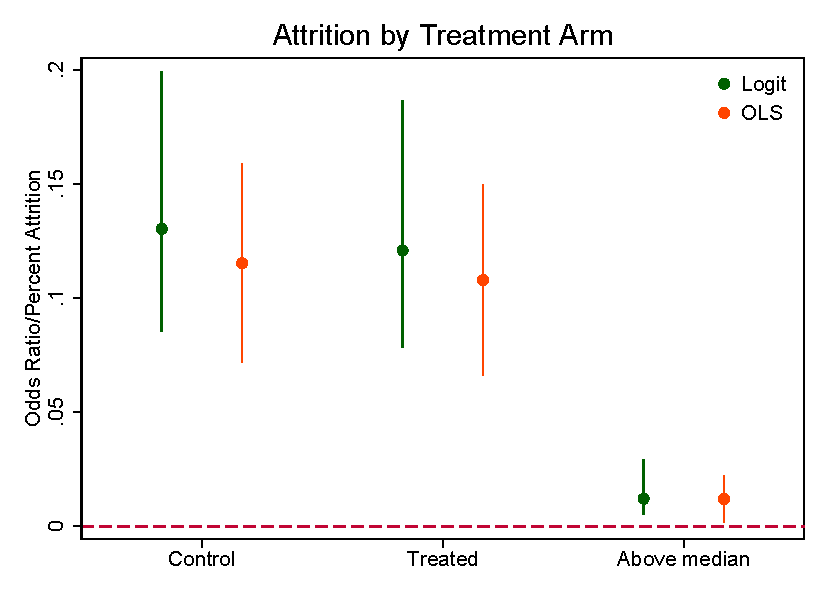
\includegraphics[width=\textwidth]{../plots/attritecoefplot.png}

%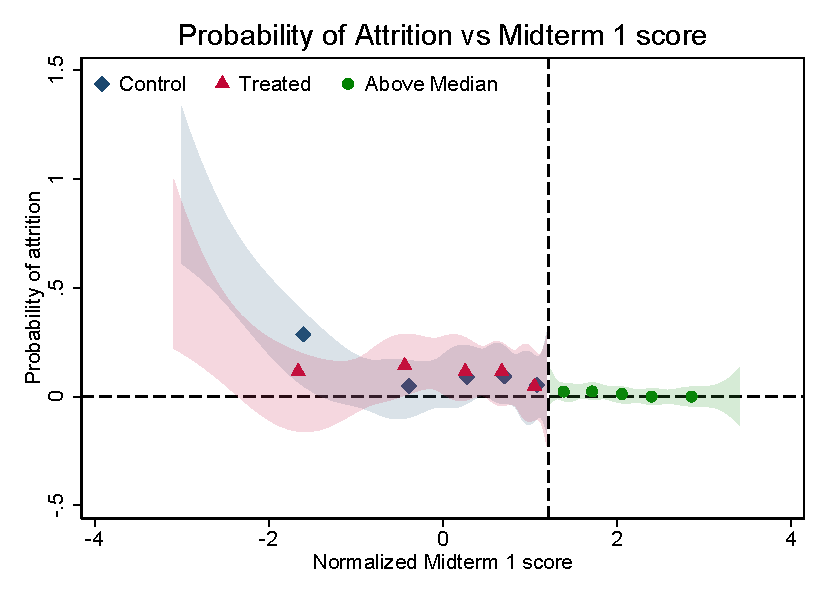
\includegraphics[width=\textwidth]{../plots/attritebinscatter.png}

%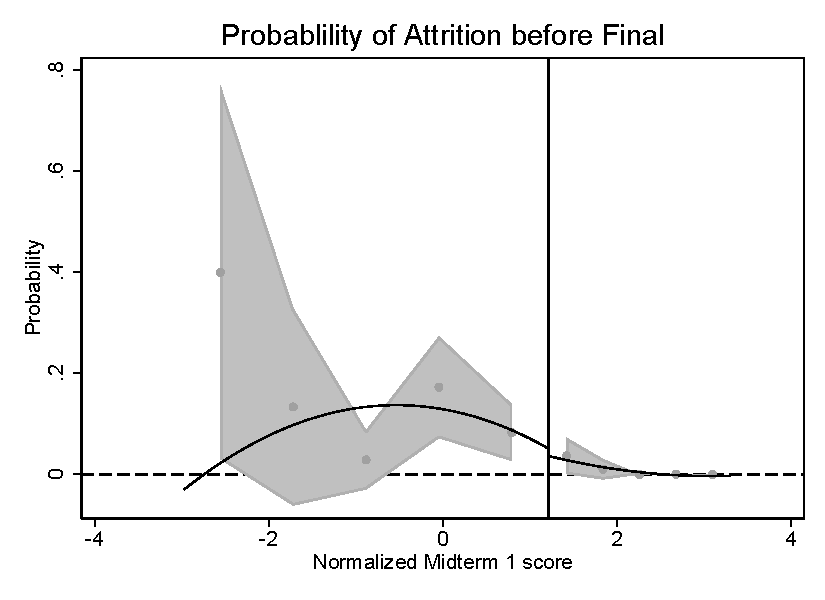
\includegraphics[width=\textwidth]{../plots/attriterd.png}

\section{Tables} \newpage

\begin{tabular}{@{\extracolsep{5pt}}lcccccccc}
\\[-1.8ex]\hline \hline \\[-1.8ex]
  & \multicolumn{2}{c}{(1)}  & \multicolumn{2}{c}{(2)}  & \multicolumn{2}{c}{(3)}  & \multicolumn{2}{c}{T-test}  \\
 & \multicolumn{2}{c}{Above median}  & \multicolumn{2}{c}{Control, All}  & \multicolumn{2}{c}{Treated, All}  & \multicolumn{2}{c}{P-value}  \\
   Variable & N & Mean/SE  & N & Mean/SE  & N & Mean/SE    & (2)-(1)   & (2)-(3)  \\ \hline \\[-1.8ex] 
Midterm 1 Score & 415 & \begin{tabular}[t]{@{}c@{}} 2.303 \\ (0.030) \end{tabular} & 184 & \begin{tabular}[t]{@{}c@{}} 0.000 \\ (0.074) \end{tabular} & 190 & \begin{tabular}[t]{@{}c@{}} -0.118 \\ (0.083) \end{tabular} &     0.000*** &     0.291 \rule{0pt}{0pt}\\
Math Quiz Score & 415 & \begin{tabular}[t]{@{}c@{}} 0.576 \\ (0.047) \end{tabular} & 184 & \begin{tabular}[t]{@{}c@{}} -0.000 \\ (0.074) \end{tabular} & 190 & \begin{tabular}[t]{@{}c@{}} 0.086 \\ (0.071) \end{tabular} &     0.000*** &     0.399 \rule{0pt}{3ex}\\
Pre Treatment Videos & 415 & \begin{tabular}[t]{@{}c@{}} 12.188 \\ (0.665) \end{tabular} & 184 & \begin{tabular}[t]{@{}c@{}} 11.739 \\ (0.821) \end{tabular} & 190 & \begin{tabular}[t]{@{}c@{}} 12.058 \\ (0.931) \end{tabular} &     0.671 &     0.798 \rule{0pt}{3ex}\\
PSET & 415 & \begin{tabular}[t]{@{}c@{}} 0.270 \\ (0.043) \end{tabular} & 184 & \begin{tabular}[t]{@{}c@{}} 0.272 \\ (0.061) \end{tabular} & 190 & \begin{tabular}[t]{@{}c@{}} 0.237 \\ (0.060) \end{tabular} &     0.980 &     0.684 \rule{0pt}{3ex}\\
Transfer Status & 412 & \begin{tabular}[t]{@{}c@{}} 0.274 \\ (0.022) \end{tabular} & 184 & \begin{tabular}[t]{@{}c@{}} 0.462 \\ (0.037) \end{tabular} & 188 & \begin{tabular}[t]{@{}c@{}} 0.447 \\ (0.036) \end{tabular} &     0.000*** &     0.770 \rule{0pt}{3ex}\\
Prev. GPA & 316 & \begin{tabular}[t]{@{}c@{}} 3.449 \\ (0.029) \end{tabular} & 118 & \begin{tabular}[t]{@{}c@{}} 2.946 \\ (0.044) \end{tabular} & 125 & \begin{tabular}[t]{@{}c@{}} 2.956 \\ (0.061) \end{tabular} &     0.000*** &     0.897 \rule{0pt}{3ex}\\
Male & 415 & \begin{tabular}[t]{@{}c@{}} 0.588 \\ (0.024) \end{tabular} & 184 & \begin{tabular}[t]{@{}c@{}} 0.647 \\ (0.035) \end{tabular} & 190 & \begin{tabular}[t]{@{}c@{}} 0.579 \\ (0.036) \end{tabular} &     0.170 &     0.179 \rule{0pt}{3ex}\\
Female & 415 & \begin{tabular}[t]{@{}c@{}} 0.390 \\ (0.024) \end{tabular} & 184 & \begin{tabular}[t]{@{}c@{}} 0.348 \\ (0.035) \end{tabular} & 190 & \begin{tabular}[t]{@{}c@{}} 0.400 \\ (0.036) \end{tabular} &     0.318 &     0.298 \rule{0pt}{3ex}\\
Other gender/not spec. & 415 & \begin{tabular}[t]{@{}c@{}} 0.014 \\ (0.006) \end{tabular} & 184 & \begin{tabular}[t]{@{}c@{}} 0.005 \\ (0.005) \end{tabular} & 190 & \begin{tabular}[t]{@{}c@{}} 0.011 \\ (0.007) \end{tabular} &     0.260 &     0.580 \rule{0pt}{3ex}\\
Chinese & 415 & \begin{tabular}[t]{@{}c@{}} 0.499 \\ (0.025) \end{tabular} & 184 & \begin{tabular}[t]{@{}c@{}} 0.500 \\ (0.037) \end{tabular} & 190 & \begin{tabular}[t]{@{}c@{}} 0.426 \\ (0.036) \end{tabular} &     0.978 &     0.154 \rule{0pt}{3ex}\\
Latinx & 415 & \begin{tabular}[t]{@{}c@{}} 0.060 \\ (0.012) \end{tabular} & 184 & \begin{tabular}[t]{@{}c@{}} 0.141 \\ (0.026) \end{tabular} & 190 & \begin{tabular}[t]{@{}c@{}} 0.153 \\ (0.026) \end{tabular} &     0.004*** &     0.758 \rule{0pt}{3ex}\\
Other Asian & 415 & \begin{tabular}[t]{@{}c@{}} 0.152 \\ (0.018) \end{tabular} & 184 & \begin{tabular}[t]{@{}c@{}} 0.141 \\ (0.026) \end{tabular} & 190 & \begin{tabular}[t]{@{}c@{}} 0.205 \\ (0.029) \end{tabular} &     0.736 &     0.102 \rule{0pt}{3ex}\\
Vietnamese & 415 & \begin{tabular}[t]{@{}c@{}} 0.046 \\ (0.010) \end{tabular} & 184 & \begin{tabular}[t]{@{}c@{}} 0.054 \\ (0.017) \end{tabular} & 190 & \begin{tabular}[t]{@{}c@{}} 0.016 \\ (0.009) \end{tabular} &     0.663 &     0.044** \rule{0pt}{3ex}\\
White & 415 & \begin{tabular}[t]{@{}c@{}} 0.149 \\ (0.018) \end{tabular} & 184 & \begin{tabular}[t]{@{}c@{}} 0.109 \\ (0.023) \end{tabular} & 190 & \begin{tabular}[t]{@{}c@{}} 0.132 \\ (0.025) \end{tabular} &     0.160 &     0.497 \rule{0pt}{3ex}\\
Other ethnicity/not spec. & 415 & \begin{tabular}[t]{@{}c@{}} 0.087 \\ (0.014) \end{tabular} & 184 & \begin{tabular}[t]{@{}c@{}} 0.054 \\ (0.017) \end{tabular} & 190 & \begin{tabular}[t]{@{}c@{}} 0.058 \\ (0.017) \end{tabular} &     0.136 &     0.882 \rule{0pt}{3ex}\\
\hline \hline \\[-1.8ex]
%%% This is the note. If it does not have the correct margins, edit text below to fit to table size.
\multicolumn{9}{@{}p{1\textwidth}}
{\textit{Notes}: Columns 1, 2, and 3 include all students who took the final exam (i.e. completed the  experiment. Columns 4 and 5 exclude students whose matched pair attrited (did not take the final).  \textit{Midterm 1 Score} and \textit{Math Quiz Score} are in standard  deviation units. \textit{Pre Treatment Videos} is the number of course-relevant  videos watched before the first midterm. \textit{PSET} is the number of visits  to the PSET tutoring lab before the first midterm. \textit{Prev. GPA} is the cumulative  GPA at the beginning of the course, which is only observed for students who had attended  UCSD previously. \textit{Transfer Status} and all gender and ethnicity variables  are binary and equal 1 if the student matches that category.  The value displayed for t-tests are p-values. Standard errors are robust. ***, **, and * indicate significance at the 1, 5, and 10 percent critical level. }
\end{tabular}


\begin{tabular}{@{\extracolsep{5pt}}lccccc}
\\[-1.8ex]\hline \hline \\[-1.8ex]
  & \multicolumn{2}{c}{(1)}  & \multicolumn{2}{c}{(2)}  & \multicolumn{1}{c}{T-test}  \\
 & \multicolumn{2}{c}{Control, All}  & \multicolumn{2}{c}{Treated, All}  & \multicolumn{1}{c}{P-value}  \\
  Variable & N & Mean/SE  & N & Mean/SE    & (1)-(2)  \\ \hline \\[-1.8ex] 
Midterm 1 Score & 166 & \begin{tabular}[t]{@{}c@{}} 0.029 \\ (0.077) \end{tabular} & 166 & \begin{tabular}[t]{@{}c@{}} 0.021 \\ (0.078) \end{tabular} &     0.938 \rule{0pt}{0pt}\\
Math Quiz Score & 166 & \begin{tabular}[t]{@{}c@{}} -0.012 \\ (0.077) \end{tabular} & 166 & \begin{tabular}[t]{@{}c@{}} 0.091 \\ (0.076) \end{tabular} &     0.341 \rule{0pt}{3ex}\\
Pre Treatment Videos & 166 & \begin{tabular}[t]{@{}c@{}} 12.090 \\ (0.882) \end{tabular} & 166 & \begin{tabular}[t]{@{}c@{}} 12.410 \\ (1.018) \end{tabular} &     0.813 \rule{0pt}{3ex}\\
PSET & 166 & \begin{tabular}[t]{@{}c@{}} 0.283 \\ (0.066) \end{tabular} & 166 & \begin{tabular}[t]{@{}c@{}} 0.253 \\ (0.066) \end{tabular} &     0.746 \rule{0pt}{3ex}\\
Transfer Status & 166 & \begin{tabular}[t]{@{}c@{}} 0.470 \\ (0.039) \end{tabular} & 164 & \begin{tabular}[t]{@{}c@{}} 0.415 \\ (0.039) \end{tabular} &     0.314 \rule{0pt}{3ex}\\
Prev. GPA & 105 & \begin{tabular}[t]{@{}c@{}} 2.929 \\ (0.047) \end{tabular} & 112 & \begin{tabular}[t]{@{}c@{}} 2.998 \\ (0.059) \end{tabular} &     0.367 \rule{0pt}{3ex}\\
Male & 166 & \begin{tabular}[t]{@{}c@{}} 0.657 \\ (0.037) \end{tabular} & 166 & \begin{tabular}[t]{@{}c@{}} 0.578 \\ (0.038) \end{tabular} &     0.143 \rule{0pt}{3ex}\\
Female & 166 & \begin{tabular}[t]{@{}c@{}} 0.337 \\ (0.037) \end{tabular} & 166 & \begin{tabular}[t]{@{}c@{}} 0.398 \\ (0.038) \end{tabular} &     0.256 \rule{0pt}{3ex}\\
Other gender/not spec. & 166 & \begin{tabular}[t]{@{}c@{}} 0.006 \\ (0.006) \end{tabular} & 166 & \begin{tabular}[t]{@{}c@{}} 0.012 \\ (0.008) \end{tabular} &     0.563 \rule{0pt}{3ex}\\
Chinese & 166 & \begin{tabular}[t]{@{}c@{}} 0.518 \\ (0.039) \end{tabular} & 166 & \begin{tabular}[t]{@{}c@{}} 0.410 \\ (0.038) \end{tabular} &     0.048** \rule{0pt}{3ex}\\
Latinx & 166 & \begin{tabular}[t]{@{}c@{}} 0.139 \\ (0.027) \end{tabular} & 166 & \begin{tabular}[t]{@{}c@{}} 0.163 \\ (0.029) \end{tabular} &     0.541 \rule{0pt}{3ex}\\
Other Asian & 166 & \begin{tabular}[t]{@{}c@{}} 0.145 \\ (0.027) \end{tabular} & 166 & \begin{tabular}[t]{@{}c@{}} 0.211 \\ (0.032) \end{tabular} &     0.115 \rule{0pt}{3ex}\\
Vietnamese & 166 & \begin{tabular}[t]{@{}c@{}} 0.048 \\ (0.017) \end{tabular} & 166 & \begin{tabular}[t]{@{}c@{}} 0.006 \\ (0.006) \end{tabular} &     0.018** \rule{0pt}{3ex}\\
White & 166 & \begin{tabular}[t]{@{}c@{}} 0.102 \\ (0.024) \end{tabular} & 166 & \begin{tabular}[t]{@{}c@{}} 0.145 \\ (0.027) \end{tabular} &     0.244 \rule{0pt}{3ex}\\
Other ethnicity/not spec. & 166 & \begin{tabular}[t]{@{}c@{}} 0.048 \\ (0.017) \end{tabular} & 166 & \begin{tabular}[t]{@{}c@{}} 0.054 \\ (0.018) \end{tabular} &     0.804 \rule{0pt}{3ex}\\
\hline \hline \\[-1.8ex]
%%% This is the note. If it does not have the correct margins, edit text below to fit to table size.
\multicolumn{6}{@{}p{1\textwidth}}
{\textit{Notes}:  The value displayed for t-tests are p-values. Standard errors are robust. ***, **, and * indicate significance at the 1, 5, and 10 percent critical level. }
\end{tabular}


\begin{table}[htbp]\centering
\def\sym#1{\ifmmode^{#1}\else\(^{#1}\)\fi}
\caption{Effect of Being Assigned Treatment (ITT) on Relevant Videos Watched}
\begin{tabular}{l*{8}{S}}
\toprule
                    &\multicolumn{4}{c}{Unique Videos}                                                      &\multicolumn{4}{c}{Total Videos}                                                       \\\cmidrule(lr){2-5}\cmidrule(lr){6-9}
                    &\multicolumn{1}{c}{All Observations}&\multicolumn{1}{c}{All Observations}&\multicolumn{1}{c}{Matching Pairs}&\multicolumn{1}{c}{Matching Pairs}&\multicolumn{1}{c}{All Observations}&\multicolumn{1}{c}{All Observations}&\multicolumn{1}{c}{Matching Pairs}&\multicolumn{1}{c}{Matching Pairs}\\
\midrule
Treated             &       21.54\sym{***}&       21.23\sym{***}&       20.51\sym{***}&       20.04\sym{***}&       39.24\sym{***}&       38.80\sym{***}&       38.29\sym{***}&       37.74\sym{***}\\
                    &      (1.55)         &      (1.31)         &      (1.39)         &      (1.43)         &      (4.06)         &      (3.14)         &      (3.42)         &      (3.60)         \\
Midterm 1 score     &       -1.40\sym{**} &       -1.32\sym{**} &       -1.15         &      -31.18         &       -2.09         &       -2.39         &       -2.91         &      -36.52         \\
                    &      (0.66)         &      (0.63)         &      (0.74)         &     (28.04)         &      (1.78)         &      (1.60)         &      (1.91)         &     (61.76)         \\
Year = 2019         &       -4.71\sym{***}&       -2.28\sym{*}  &       -2.88\sym{**} &                     &      -12.78\sym{***}&       -6.41\sym{*}  &       -7.98\sym{**} &                     \\
                    &      (1.53)         &      (1.26)         &      (1.34)         &                     &      (4.05)         &      (3.27)         &      (3.63)         &                     \\
Intercept           &       36.39\sym{***}&       12.72\sym{*}  &       14.02\sym{**} &        7.05         &       59.71\sym{***}&      -18.68         &      -19.59         &      -47.32\sym{*}  \\
                    &      (1.59)         &      (6.96)         &      (6.95)         &     (10.13)         &      (4.10)         &     (12.98)         &     (14.04)         &     (24.20)         \\
\midrule
N                   &\multicolumn{1}{c}{374}         &\multicolumn{1}{c}{372}         &\multicolumn{1}{c}{330}         &\multicolumn{1}{c}{330}         &\multicolumn{1}{c}{374}         &\multicolumn{1}{c}{372}         &\multicolumn{1}{c}{330}         &\multicolumn{1}{c}{330}         \\
Controls            &        {No}         &       {Yes}         &       {Yes}         &       {Yes}         &        {No}         &       {Yes}         &       {Yes}         &       {Yes}         \\
Pair Fixed Effects  &        {No}         &        {No}         &        {No}         &       {Yes}         &        {No}         &        {No}         &        {No}         &       {Yes}         \\
\bottomrule \multicolumn{9}{@{}p{1\textwidth}} {\textit{Notes}: 'Videos watched' includes all videos watched before the final exam relevant to the course. Test score variables are normalized by the control mean and standard deviation. Standard errors are robust to heteroskedasticity. ***, **, and * indicate significance at the 1, 5, and 10 percent critical levels, respectively.} \end{tabular} \end{table}


\begin{table}[htbp]\centering
\def\sym#1{\ifmmode^{#1}\else\(^{#1}\)\fi}
\caption{Effect of Being Assigned Treatment (ITT) on Relevant Videos Watched before Midterm 2}
\begin{tabular}{l*{8}{S}}
\toprule
                    &\multicolumn{4}{c}{Unique Videos}                                                      &\multicolumn{4}{c}{Total Videos}                                                       \\\cmidrule(lr){2-5}\cmidrule(lr){6-9}
                    &\multicolumn{1}{c}{All Observations}&\multicolumn{1}{c}{All Observations}&\multicolumn{1}{c}{Matching Pairs}&\multicolumn{1}{c}{Matching Pairs}&\multicolumn{1}{c}{All Observations}&\multicolumn{1}{c}{All Observations}&\multicolumn{1}{c}{Matching Pairs}&\multicolumn{1}{c}{Matching Pairs}\\
\midrule
Treated             &        6.74\sym{***}&        6.05\sym{***}&        6.01\sym{***}&        5.19\sym{***}&       10.26\sym{***}&        9.60\sym{***}&        9.68\sym{***}&        8.19\sym{***}\\
                    &      (1.56)         &      (1.12)         &      (1.19)         &      (1.29)         &      (2.82)         &      (1.80)         &      (1.96)         &      (1.96)         \\
Midterm 1 score     &        0.01         &       -0.25         &       -0.72         &      -43.51         &       -0.51         &       -0.72         &       -1.69         &      -68.41\sym{*}  \\
                    &      (0.72)         &      (0.63)         &      (0.69)         &     (28.68)         &      (1.29)         &      (0.95)         &      (1.10)         &     (40.92)         \\
Year = 2019         &       -8.76\sym{***}&       -5.95\sym{***}&       -6.89\sym{***}&                     &      -13.51\sym{***}&       -8.03\sym{***}&       -9.29\sym{***}&                     \\
                    &      (1.57)         &      (1.16)         &      (1.20)         &                     &      (2.84)         &      (1.80)         &      (1.96)         &                     \\
Intercept           &       26.23\sym{***}&        2.49         &        3.59         &       -5.19         &       38.23\sym{***}&       -7.26         &       -5.58         &      -18.56         \\
                    &      (1.38)         &      (7.22)         &      (7.42)         &     (14.83)         &      (2.55)         &      (9.25)         &      (9.56)         &     (18.11)         \\
\midrule
N                   &\multicolumn{1}{c}{374}         &\multicolumn{1}{c}{374}         &\multicolumn{1}{c}{332}         &\multicolumn{1}{c}{332}         &\multicolumn{1}{c}{374}         &\multicolumn{1}{c}{374}         &\multicolumn{1}{c}{332}         &\multicolumn{1}{c}{332}         \\
Controls            &        {No}         &       {Yes}         &       {Yes}         &       {Yes}         &        {No}         &       {Yes}         &       {Yes}         &       {Yes}         \\
Pair Fixed Effects  &        {No}         &        {No}         &        {No}         &       {Yes}         &        {No}         &        {No}         &        {No}         &       {Yes}         \\
\bottomrule \multicolumn{9}{@{}p{1\textwidth}} {\textit{Notes}: 'Videos watched' includes all videos watched before the second midterm relevant to the course. Test score variables are normalized by the control mean and standard deviation. Standard errors are robust to heteroskedasticity. ***, **, and * indicate significance at the 1, 5, and 10 percent critical levels, respectively.} \end{tabular} \end{table}


\begin{table}[htbp]\centering
\def\sym#1{\ifmmode^{#1}\else\(^{#1}\)\fi}
\caption{Effect of Being Assigned Treatment (ITT) on Duration of Videos Wathced}
\begin{tabular}{l*{8}{S}}
\toprule
                    &\multicolumn{4}{c}{Unique Videos}                                                      &\multicolumn{4}{c}{Total Videos}                                                       \\\cmidrule(lr){2-5}\cmidrule(lr){6-9}
                    &\multicolumn{1}{c}{All Observations}&\multicolumn{1}{c}{All Observations}&\multicolumn{1}{c}{Matching Pairs}&\multicolumn{1}{c}{Matching Pairs}&\multicolumn{1}{c}{All Observations}&\multicolumn{1}{c}{All Observations}&\multicolumn{1}{c}{Matching Pairs}&\multicolumn{1}{c}{Matching Pairs}\\
\midrule
Treated             &        2.24\sym{***}&        2.22\sym{***}&        2.17\sym{***}&        2.12\sym{***}&        4.09\sym{***}&        4.05\sym{***}&        4.08\sym{***}&        4.10\sym{***}\\
                    &      (0.27)         &      (0.25)         &      (0.27)         &      (0.29)         &      (0.50)         &      (0.41)         &      (0.44)         &      (0.53)         \\
Midterm 1 score     &       -0.16         &       -0.15         &       -0.32\sym{*}  &       -9.11         &       -0.15         &       -0.20         &       -0.28         &        0.84         \\
                    &      (0.17)         &      (0.16)         &      (0.19)         &      (7.13)         &      (0.29)         &      (0.25)         &      (0.28)         &     (15.34)         \\
Year = 2019         &        0.39         &        0.71\sym{***}&        0.67\sym{**} &                     &       -0.02         &        0.70\sym{*}  &        0.69         &                     \\
                    &      (0.27)         &      (0.25)         &      (0.27)         &                     &      (0.50)         &      (0.41)         &      (0.45)         &                     \\
Intercept           &        3.68\sym{***}&        3.29\sym{***}&        3.17\sym{***}&        5.53\sym{***}&        5.79\sym{***}&        1.96         &        1.14         &        5.69\sym{***}\\
                    &      (0.24)         &      (1.08)         &      (1.17)         &      (1.29)         &      (0.45)         &      (1.59)         &      (1.74)         &      (2.14)         \\
\midrule
N                   &\multicolumn{1}{c}{395}         &\multicolumn{1}{c}{395}         &\multicolumn{1}{c}{331}         &\multicolumn{1}{c}{331}         &\multicolumn{1}{c}{395}         &\multicolumn{1}{c}{395}         &\multicolumn{1}{c}{362}         &\multicolumn{1}{c}{362}         \\
Controls            &        {No}         &       {Yes}         &       {Yes}         &        {No}         &        {No}         &       {Yes}         &       {Yes}         &        {No}         \\
Pair Fixed Effects  &        {No}         &        {No}         &        {No}         &       {Yes}         &        {No}         &        {No}         &        {No}         &       {Yes}         \\
\bottomrule \multicolumn{9}{@{}p{1\textwidth}} {\textit{Notes}: 'Videos watched' includes all videos watched before the second midterm relevant to the course. Test score variables are normalized by the control mean and standard deviation. Standard errors are robust to heteroskedasticity. ***, **, and * indicate significance at the 1, 5, and 10 percent critical levels, respectively.} \end{tabular} \end{table}


\begin{table}[htbp]\centering
\def\sym#1{\ifmmode^{#1}\else\(^{#1}\)\fi}
\caption{Effect of Being Assigned Treatment (ITT) on Test Scores}
\begin{tabular}{l*{8}{S}}
\toprule
                    &\multicolumn{3}{c}{Final}                                        &\multicolumn{5}{c}{Midterm 2}                                                                                \\\cmidrule(lr){2-4}\cmidrule(lr){5-9}
                    &\multicolumn{1}{c}{All Observations}&\multicolumn{1}{c}{Matching Pairs}&\multicolumn{1}{c}{Matching Pairs}&\multicolumn{1}{c}{All Observations}&\multicolumn{1}{c}{Matching Pairs}&\multicolumn{1}{c}{Matching Pairs}&\multicolumn{1}{c}{mid23}&\multicolumn{1}{c}{mid24}\\
\midrule
Treated             &        0.17\sym{**} &        0.13         &        0.10         &        0.07         &        0.23\sym{**} &        0.18\sym{**} &        0.17\sym{*}  &        0.12         \\
                    &      (0.09)         &      (0.09)         &      (0.09)         &      (0.11)         &      (0.09)         &      (0.09)         &      (0.10)         &      (0.10)         \\
Midterm 1 score     &        0.53\sym{***}&        0.43\sym{***}&        0.41\sym{***}&        0.88         &        0.49\sym{***}&        0.39\sym{***}&        0.37\sym{***}&        0.25         \\
                    &      (0.04)         &      (0.04)         &      (0.05)         &      (1.77)         &      (0.04)         &      (0.04)         &      (0.05)         &      (2.06)         \\
Year = 2019         &        0.01         &        0.02         &        0.00         &                     &        0.07         &        0.06         &        0.05         &                     \\
                    &      (0.09)         &      (0.09)         &      (0.10)         &                     &      (0.09)         &      (0.09)         &      (0.10)         &                     \\
Intercept           &       -0.00         &       -1.13\sym{*}  &       -1.16\sym{*}  &       -0.79         &       -0.04         &       -1.61\sym{*}  &       -1.73\sym{*}  &       -0.87         \\
                    &      (0.08)         &      (0.63)         &      (0.62)         &      (0.69)         &      (0.08)         &      (0.90)         &      (0.91)         &      (0.80)         \\
\midrule
\multicolumn{1}{c}{N}&\multicolumn{1}{c}{374}         &\multicolumn{1}{c}{374}         &\multicolumn{1}{c}{332}         &\multicolumn{1}{c}{332}         &\multicolumn{1}{c}{373}         &\multicolumn{1}{c}{373}         &\multicolumn{1}{c}{331}         &\multicolumn{1}{c}{331}         \\
\bottomrule \multicolumn{9}{@{}p{1\textwidth}} {\textit{Notes}: Test score variables are in standard deviation-units. Standard errors are robust to heteroskedasticity. ***, **, and * indicate significance at the 1, 5, and 10 percent critical levels, respectively.} \end{tabular} \end{table}


\begin{table}[htbp]\centering
\def\sym#1{\ifmmode^{#1}\else\(^{#1}\)\fi}
\caption{Effect of Watching Videos (LATE) on Test Scores for those induced by treatment}
\begin{tabular}{l*{8}{S}}
\toprule
                    &\multicolumn{3}{c}{Final}                                        &\multicolumn{5}{c}{Midterm 2}                                                                                \\\cmidrule(lr){2-4}\cmidrule(lr){5-9}
                    &\multicolumn{1}{c}{All Observations}&\multicolumn{1}{c}{Matching Pairs}&\multicolumn{1}{c}{Matching Pairs}&\multicolumn{1}{c}{All Observations}&\multicolumn{1}{c}{Matching Pairs}&\multicolumn{1}{c}{Matching Pairs}&\multicolumn{1}{c}{m7}&\multicolumn{1}{c}{m8}\\
\midrule
relu\_since\_mid1     &                     &                     &                     &                     &                     &                     &                     &                     \\
                    &                     &                     &                     &                     &                     &                     &                     &                     \\
relu\_bt\_mid1\_mid2   &                     &                     &                     &                     &                     &                     &                     &                     \\
                    &                     &                     &                     &                     &                     &                     &                     &                     \\
Unique, relevant videos&       0.008\sym{**} &       0.006         &       0.005         &       0.003         &                     &                     &                     &                     \\
                    &     (0.004)         &     (0.004)         &     (0.004)         &     (0.005)         &                     &                     &                     &                     \\
Midterm 1 score     &       0.538\sym{***}&       0.439\sym{***}&       0.420\sym{***}&                     &       0.491\sym{***}&       0.398\sym{***}&       0.392\sym{***}&                     \\
                    &     (0.039)         &     (0.041)         &     (0.048)         &                     &     (0.044)         &     (0.045)         &     (0.053)         &                     \\
Year = 2019         &       0.047         &       0.030         &       0.018         &                     &       0.377\sym{**} &       0.237\sym{*}  &       0.241\sym{*}  &                     \\
                    &     (0.090)         &     (0.088)         &     (0.093)         &                     &     (0.166)         &     (0.123)         &     (0.143)         &                     \\
Unique, rel. videos before Midterm 2&                     &                     &                     &                     &       0.035\sym{**} &       0.030\sym{**} &       0.028\sym{*}  &       0.021         \\
                    &                     &                     &                     &                     &     (0.015)         &     (0.015)         &     (0.016)         &     (0.019)         \\
Intercept           &      -0.299         &      -1.205\sym{**} &      -1.235\sym{**} &                     &      -0.947\sym{**} &      -1.502\sym{*}  &      -1.662\sym{*}  &                     \\
                    &     (0.202)         &     (0.601)         &     (0.595)         &                     &     (0.454)         &     (0.839)         &     (0.866)         &                     \\
\midrule
\multicolumn{1}{c}{N}&\multicolumn{1}{c}{374}         &\multicolumn{1}{c}{374}         &\multicolumn{1}{c}{332}         &\multicolumn{1}{c}{332}         &\multicolumn{1}{c}{373}         &\multicolumn{1}{c}{373}         &\multicolumn{1}{c}{331}         &\multicolumn{1}{c}{330}         \\
\bottomrule \multicolumn{7}{@{}p{1\textwidth}} {\textit{Notes}: 'Unique relevant video' variables are instrumented using exogenously assigned treatment. The first coefficient in each column is the local average treatment effect of each video that was induced to be watched by treatment. Test score variables are in standard deviation-units. Standard errors are robust to heteroskedasticity. ***, **, and * indicate significance at the 1, 5, and 10 percent critical levels, respectively.} \end{tabular} \end{table}


\begin{table}[htbp] \centering \begin{threeparttable} \def\sym#1{\ifmmode^{#1}\else\(^{#1}\)\fi} \caption{Interaction effect coefficients: first stage} \begin{tabular}{l*{4}{c}} \toprule 
                    &\multicolumn{1}{c}{(1)}&\multicolumn{1}{c}{(2)}&\multicolumn{1}{c}{(3)}&\multicolumn{1}{c}{(4)}\\
                    &\multicolumn{1}{c}{Unique, relevant videos}&\multicolumn{1}{c}{Unique, relevant videos}&\multicolumn{1}{c}{Relevant videos}&\multicolumn{1}{c}{Relevant videos}\\
\midrule
Treated $\times$ Midterm 1 score&       1.520         &       0.504         &       2.563         &      -0.468         \\
                    &     (1.759)         &     (1.655)         &     (4.412)         &     (3.754)         \\
[1em]
Treated $\times$ Math Quiz score&       0.703         &      -0.474         &      -1.357         &      -4.722         \\
                    &     (1.962)         &     (1.678)         &     (4.291)         &     (3.499)         \\
[1em]
Treated $\times$ PSET&       0.540         &      -1.398         &      -3.612         &      -9.931         \\
                    &     (1.783)         &     (1.536)         &     (7.186)         &     (5.441)         \\
[1em]
Treated $\times$ Freshman&       3.459         &       3.255         &      -0.539         &      -1.138         \\
                    &     (3.063)         &     (2.576)         &     (8.075)         &     (6.282)         \\
[1em]
Treated $\times$ Transfer Student&      -2.872         &      -3.006         &       1.601         &       1.288         \\
                    &     (3.065)         &     (2.573)         &     (8.065)         &     (6.256)         \\
[1em]
Treated $\times$ Male&      -2.242         &      -1.235         &      -8.081         &      -5.034         \\
                    &     (3.172)         &     (2.651)         &     (8.213)         &     (6.320)         \\
[1em]
Treated $\times$ Female&       2.139         &       0.843         &       8.575         &       4.590         \\
                    &     (3.190)         &     (2.683)         &     (8.250)         &     (6.392)         \\
[1em]
Treated $\times$ Asian&       2.686         &       3.279         &       4.244         &       5.422         \\
                    &     (3.254)         &     (2.781)         &     (8.652)         &     (6.415)         \\
[1em]
Treated $\times$ Latinx&      -8.336\sym{*}  &      -5.193         &      -5.822         &       4.524         \\
                    &     (3.602)         &     (3.316)         &     (9.177)         &     (8.865)         \\
[1em]
Treated $\times$ White&       6.144         &       2.305         &       9.539         &      -1.255         \\
                    &     (4.658)         &     (3.673)         &    (13.091)         &     (8.249)         \\
[1em]
Treated $\times$ Other ethnicity/not spec.&      -3.609         &      -5.653         &     -22.910         &     -31.190         \\
                    &     (7.034)         &     (5.891)         &    (22.922)         &    (15.895)         \\
\midrule
Observations        &         374         &         374         &         374         &         374         \\
\bottomrule \end{tabular} \begin{tablenotes} \item \textit{Notes}: Each coefficient is the estimated $\beta_3$ from equation (X). Test score (outcome) variables are in standard deviation units. Standard errors are robust to heteroskedasticity. ***, **, and * indicate significance at the 1, 5, and 10 percent critical levels, respectively. \end{tablenotes} \end{threeparttable} \end{table}


\begin{table}[htbp] \centering \begin{threeparttable} \def\sym#1{\ifmmode^{#1}\else\(^{#1}\)\fi} \caption{Interaction effect coefficients: second stage} \begin{tabular}{l*{4}{c}} \toprule 
                    &\multicolumn{1}{c}{(1)}&\multicolumn{1}{c}{(2)}&\multicolumn{1}{c}{(3)}&\multicolumn{1}{c}{(4)}\\
                    &\multicolumn{1}{c}{Final exam score}&\multicolumn{1}{c}{Final exam score}&\multicolumn{1}{c}{Midterm 2 score}&\multicolumn{1}{c}{Midterm 2 score}\\
\midrule
Treated $\times$ Midterm 1 score&       0.002         &      -0.056         &       0.009         &      -0.006         \\
                    &     (0.095)         &     (0.100)         &     (0.086)         &     (0.093)         \\
[1em]
Treated $\times$ Math Quiz score&       0.090         &       0.076         &       0.165         &       0.161         \\
                    &     (0.100)         &     (0.096)         &     (0.102)         &     (0.099)         \\
[1em]
Treated $\times$ PSET&      -0.046         &      -0.023         &      -0.027         &       0.007         \\
                    &     (0.110)         &     (0.097)         &     (0.100)         &     (0.096)         \\
[1em]
Treated $\times$ Freshman&      -0.178         &      -0.216         &       0.129         &       0.134         \\
                    &     (0.177)         &     (0.173)         &     (0.183)         &     (0.177)         \\
[1em]
Treated $\times$ Transfer Student&       0.130         &       0.171         &      -0.139         &      -0.139         \\
                    &     (0.178)         &     (0.173)         &     (0.183)         &     (0.176)         \\
[1em]
Treated $\times$ Male&       0.239         &       0.323         &       0.153         &       0.192         \\
                    &     (0.187)         &     (0.183)         &     (0.185)         &     (0.187)         \\
[1em]
Treated $\times$ Female&      -0.322         &      -0.382\sym{*}  &      -0.208         &      -0.238         \\
                    &     (0.188)         &     (0.184)         &     (0.185)         &     (0.187)         \\
[1em]
Treated $\times$ Asian&      -0.215         &      -0.231         &      -0.402\sym{*}  &      -0.440\sym{*}  \\
                    &     (0.180)         &     (0.171)         &     (0.189)         &     (0.178)         \\
[1em]
Treated $\times$ Latinx&       0.022         &       0.069         &       0.237         &       0.264         \\
                    &     (0.227)         &     (0.223)         &     (0.254)         &     (0.232)         \\
[1em]
Treated $\times$ White&       0.271         &       0.335         &       0.638\sym{*}  &       0.713\sym{**} \\
                    &     (0.250)         &     (0.231)         &     (0.260)         &     (0.247)         \\
[1em]
Treated $\times$ Other ethnicity/not spec.&       0.276         &       0.112         &      -0.113         &      -0.271         \\
                    &     (0.347)         &     (0.318)         &     (0.307)         &     (0.317)         \\
\midrule
Observations        &         374         &         374         &         395         &         395         \\
\bottomrule \end{tabular} \begin{tablenotes} \item \textit{Notes}: Each coefficient is the estimated $\beta_3$ from equation (X). Test score (outcome) variables are in standard deviation units. Standard errors are robust to heteroskedasticity. ***, **, and * indicate significance at the 1, 5, and 10 percent critical levels, respectively. \end{tablenotes} \end{threeparttable} \end{table}


%\section{Appendix}

%\includegraphics[width=\textwidth]{./plots/ppopbar.png}


%\input{./firststage_pre_mid1_table.tex}

\end{document}